\documentclass{article}
\usepackage{graphicx}
\usepackage{hyperref}
\usepackage{caption}
\usepackage{subcaption}
\usepackage[dutch]{babel}

\begin{document}

\begin{center}
	\huge{Wiskunde in Kunst}\\
	\LARGE{Opdracht 4} \\
	
	\vspace{2cm}
	
	\Large{Chaostheorie}\\
	
	\vfill
	
	\begin{figure}[Hh]
		\centering
		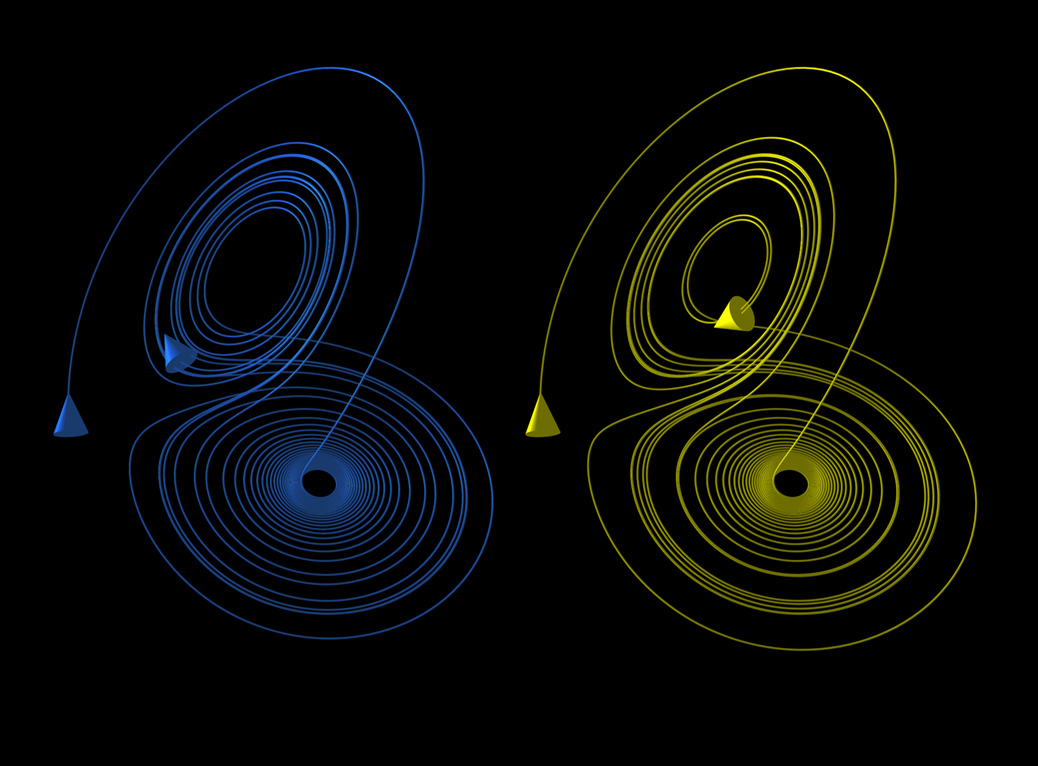
\includegraphics[width=\textwidth]{TwoLorenzOrbits}
		\label{}
	\end{figure}
	
	\vfill
	\Large{Marcelo Dias Avelino} \hfill \large{0840416}
\end{center}

\pagebreak

\section{Wat is de chaostheorie?}

De chaostheorie is een wiskundig gebied waarin het gedrag van bepaalde dynamische systemen worden onderzocht. 

Een dynamische systeem is een systeem met geheugen en het gedrag van het systeem wordt volledig door wat er in het geheugen zit en door de invloed van de omgeving bepaald. Het geheugen heet de toestand van het systeem en het wordt beschreven met getallen. Dit soort systemen zijn onderverdeeld in zo genaamd orde systemen. Dit betekent dat bij een eerste-ordersysteem het geheugen maar één stap ver gaat, twee stappen bij een tweede-ordersysteem, enzovoort. Een voorbeeld van een eerste-ordersysteem is een leeglopend bad; het enige stap dat het neemt is het leeglopen van het water. Een tweede-ordesysteem neemt, zoals eerder uitgelegd, twee stappen en is daarom beschreven door twee getallen. Een bekende voorbeeld van zo een systeem is een gewicht die op een veer rust. De twee stappen zijn dan de snelheid van het gewicht en de uitrekking van de veer. 

\pagebreak

\begin{thebibliography}{9}

\bibitem{}
	\url{http://en.wikipedia.org/wiki/Circle_Limit_III}

\bibitem{}
	\url{http://nl.wikipedia.org/wiki/Hyperbolische_meetkunde}

\bibitem{}
	\url{http://en.wikipedia.org/wiki/Hyperbolic_geometry}

\bibitem{}
	\url{http://en.wikipedia.org/wiki/Wallpaper_group}

\bibitem{}
	\url{http://en.wikipedia.org/wiki/Tessellation}

\bibitem{}
	\url{http://nl.wikipedia.org/wiki/Betegeling}

\bibitem{}
	\url{http://nl.wikipedia.org/wiki/Houtsnede}

\bibitem{}
	\url{http://en.wikipedia.org/wiki/Non-Euclidean_geometry}

\bibitem{}
	\url{http://nl.wikipedia.org/wiki/Niet-euclidische_meetkunde}

\bibitem{}
	\url{http://nl.wikipedia.org/wiki/Maurits_Cornelis_Escher}

\bibitem{}
	\url{http://en.wikipedia.org/wiki/M._C._Escher}

\bibitem{}
	\url{http://en.wikipedia.org/wiki/Baarn}

\bibitem{}
	\url{http://nl.wikipedia.org/wiki/Donald_Coxeter}

	
\end{thebibliography}

\end{document}
